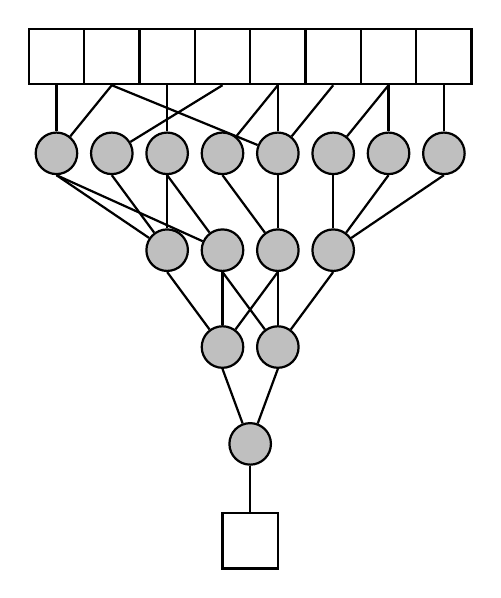
\begin{tikzpicture}[
	net node/.style = {draw, thick},
	port/.style = {net node, rectangle, minimum size=2em},
	neuron/.style = {net node, circle, minimum size=1.5em, fill=gray!50!white},
	edge/.style = {thick},
]

	%% The input row (index = 1)
	\begin{scope}
		%% Iterate from 1-8, storing the index in \n
		\foreach \n in {1,...,8}{%
			\node [port] at (\n*2em, 0) (1-\n) {};
		}
	\end{scope}

	%% Iterate through the processing rows
	%% We use a counter to track the row number
	\foreach [count=\r from 2] \m in {8, 4, 2, 1}{%
		%% Calculate the shifts using PGF math
		\pgfmathsetmacro\xShift{(8-\m)/2*2em}
		\pgfmathsetmacro\yShift{(\r-1)*-3.5em}

		\begin{scope}[xshift=\xShift, yshift=\yShift]
			\foreach \n in {1,...,\m}{%
				\node [neuron] at (\n*2em, 0) (\r-\n) {};
			}
		\end{scope}
	}

	%% The output row
	\node at (9em,-17.5em) [port] (6-1) {};

	%% Draw the connections
	%% User specified
	\foreach [count=\m] \l in {%
		{1/1, 2/1, 2/5, 3/3, 4/2, 5/4, 5/5, 6/5, 7/6, 7/7, 8/8},	% 1st to 2nd
		{1/1, 1/2, 2/1, 3/1, 3/2, 4/3, 5/3, 6/4, 7/4, 8/4},		% 2nd to 3rd
		{1/1, 2/1, 2/2, 3/1, 3/2, 4/2},					% 3rd to 4th
	}{%
		%% \m is the start row, let \n be the end row
		\pgfmathtruncatemacro\n{\m+1}	% Truncate makes an int from a float
	
		\foreach \u/\v in \l {% Here \l is one of the lists defined above
			\draw [edge] (\m-\u.south) to (\n-\v);
		}
	}

	%% Always present
	\foreach [count=\m from 4] \l in {{1/1, 2/1}, {1/1}}{%
		\pgfmathtruncatemacro\n{\m+1}	% Truncate makes an int from a float
		\foreach \u/\v in \l {% Here \l is one of the lists defined above
			\draw [edge] (\m-\u.south) to (\n-\v);
		}
	}

\end{tikzpicture}
